\chapter{Metodologia} \label{metodologia}

A metodologia para o desenvolvimento do compilador proposto adota uma abordagem prática, estruturada em etapas principais: a análise de informações relevantes sobre BRDFs e a compilação de \textit{shaders}; a exploração de técnicas existentes no domínio; a especificação da linguagem de entrada, um subconjunto de \LaTeX{}; a implementação do compilador; e a avaliação de seu desempenho por meio de experimentos de renderização.

O método para realizar a análise e a exploração de técnicas é descrito na \autoref{analise}. Em seguida, a especificação da linguagem de entrada é apresentada na \autoref{especificacao-linguagem}. É importante destacar que a definição formal da gramática está consolidada no capítulo de desenvolvimento, na \autoref{section-parser}.

Posteriormente, é discutida a elaboração dos casos de teste para validar a correção e a precisão do compilador, conforme detalhado na \autoref{testes}. Embora a validação escolhida se baseie nesses testes iniciais, os resultados obtidos no \autoref{chapter.resultados} expandem a validação para um conjunto maior de BRDFs.

O método de implementação do compilador é detalhado na \autoref{compiladorimplementacao}, enquanto a avaliação dos experimentos de renderização, focada na qualidade visual dos \textit{shaders} compilados, é exposta na \autoref{experimentos-renderizacao}.

% A \autoref{experimentos-renderizacao} planeja o método de avaliação dos experimentos de renderização quanto a qualidade visual dos \textit{shaders} compilados.

Seguindo essa metodologia, a ferramenta proposta busca compilar descrições de BRDFs em \textit{shaders} GLSL, garantindo qualidade e precisão no resultado final.

% Posteriormente, uma ideia de como o \textit{design} dos casos de teste devem ser elaborados para validar a correção e precisão do compilador é apresentado na \autoref{testes}, apesar do metódo escolhido foi os testes que mostrando, os resultados expandem esses testes e testamos mais brdfs ainda no \autoref{chapter.resultado}. O método de implementação do compilador é detalhado na \autoref{compiladorimplementacao}. Seguindo essa metodologia, a ferramenta proposta visa compilar efetivamente descrições de BRDF em \textit{shaders} GLSL.



\section{Análise e Técnicas} \label{analise}


O primeiro passo envolve a realização de uma análise detalhada das áreas relacionadas ao desenvolvimento da ferramenta proposta. Isso inclui a revisão da literatura (\autoref{revisao}) sobre BRDFs, linguagens de \textit{shaders}, \textit{design} de compiladores e técnicas de renderização gráfica. Além disso, envolve o estudo de ferramentas e bibliotecas pertinentes.

Durante essa análise, foram estudados conceitos de radiometria para compreender tecnicamente as BRDFs. A principal fonte de informação sobre radiância e BRDFs foi o livro ``Physically Based Rendering: From Theory To Implementation'' \cite{pbr}. Esse livro foi importante para compreensão da equação de renderização (\autoref{eq-rendering-equation}).

A leitura de exemplos práticos, presentes no código-fonte e nos \textit{shaders} da ferramenta discutida na \autoref{experimentos-renderizacao}, permitiu a familiarização com o desenvolvimento de BRDFs, fornecendo uma base sólida para compreender o mapeamento de equações para código, aspecto essencial para o desenvolvimento do compilador proposto neste trabalho.

Além disso, foram exploradas algumas técnicas de compilação, o que levou à escolha do método de Pratt \textit{Parsing} para a construção do compilador. Também foram estudados conceitos de recursividade e caminhada em árvores, que foram aplicados na análise semântica e na geração de código.


\section{Especificação da Linguagem}\label{especificacao-linguagem}

As especificações da linguagem de entrada para o compilador é definida. A linguagem de entrada é uma versão simplificada do \LaTeX{}, na qual as expressões matemáticas em ambientes \texttt{equation} são suficientes para descrever BRDFs. O \LaTeX{}  é um sistema de composição amplamente utilizado para documentos matemáticos e científicos. O ambiente \texttt{equation} é especificamente projetado para exibir equações individuais. O \autoref{equation-latex} é um exemplo de código-fonte \LaTeX{}  usando o ambiente \texttt{equation}.


\begin{codigo}[H]
\caption{\small Código-fonte de função quadrática.}
\label{equation-latex}
\begin{lstlisting}
\begin{equation}
    g(x) = ax^2 + bx + c
\end{equation}
\end{lstlisting}
\end{codigo}




Este código representa a equação quadrática \( g(x) = ax^2 + bx + c \), onde \( a \), \( b \) e \( c \) são coeficientes. O código GLSL correspondente gerado a partir dessa equação pode ser o \autoref{cod-glsl-g}.

\begin{codigo}[H]
\caption{\small Código GLSL da função quadrática g.}
\label{cod-glsl-g}
\begin{lstlisting}
float g(float x, float a, float b, float c) {
    return a * x * x + b * x + c;
}
\end{lstlisting}
\end{codigo}

O ambiente de equações do \LaTeX{} oferece uma ampla gama de construções matemáticas, mas, para este projeto, é necessário restringir-se a um subconjunto essencial para representar BRDFs. Ao analisar as principais BRDFs, como as citadas na \autoref{testes}, identificam-se construções indispensáveis que devem ser reconhecidas e interpretadas pelo compilador para gerar código GLSL, como as apresentadas na \autoref{tab-definition-of-lang}.

\begin{table}[htbp]
\centering
\begin{tabular}{|l|l|l|}
% \begin{tabularx}{\textwidth}{|L|L|L|}
\hline
    \textbf{Descrição} & \textbf{Exemplos} & \textbf{Comando \LaTeX{}} \\ \hline

    \small Funções trigonométricas & $\tan, \sin, \cos$ {\small e suas funções inversas}
    &\small\verb"\tan", \verb"\sin", \verb"\cos"
    \newline\verb"\arctan", \verb"\arcsin", $\dots$
    \\ \hline
\small Função raiz quadrada & $\sqrt{}$ & \verb|\sqrt| \\ \hline
\small Função exponencial & $\exp{}$ & \verb|\exp| \\ \hline
\small Funções utilitárias & $\max, \min$ & \verb|\max, \min| \\ \hline
\small Definições de equações & $f = x$ & \verb|f = x| \\ \hline
\small Definições de funções & $f(x, y) = x^y$ & \verb|f(x, y) = x^y| \\ \hline
\small Constantes comuns & $\pi$, $\epsilon$ & \verb|\pi, \epsilon| \\ \hline
\small Constantes de radiometria & $\theta_i$ {\small e outras presentes na \autoref{tab-conventions-metodologia}} & \verb|\theta_i| \\ \hline
\small Indicadores de vetor & $\vec{n}$ & \verb|\vec{}| \\ \hline
\small Identificadores aninhados & $f_{n_{i}}$ & \verb|f_{n_{i}}| \\ \hline
\small Chamadas de funções & $f(x + y)$ & \verb|f(x + y)| \\ \hline
\small Produto vetorial & $x \times y$ & \verb|x \times y| \\ \hline
\small Soma e Subtração & $x + y$, $x - y$ & \verb|x + y|, \verb|x - y| \\ \hline
\small Negação & $-y$ & \verb|-y| \\ \hline
\small Multiplicação & $x \cdot y$ & \verb|x \cdot y| \\ \hline
\small Frações & $\frac{x}{y}$ & \verb|\frac{x}{y}| \\ \hline
\small Divisão & $x / y$ & \verb|x / y| \\ \hline
\small Potenciação & $x^y$ & \verb|x^y| \\ \hline
\end{tabular}
\caption{Tabela de especificação da linguagem.}
\label{tab-definition-of-lang}
\end{table}

A descrição completa dos símbolos reconhecidos em nível de código está na seção dedicada ao \textit{lexer} (\autoref{section-lexer}), enquanto a gramática completa reconhecida pelo compilador é apresentada na seção sobre o \textit{parser} (\autoref{section-parser}).

Embora o \textit{lexer} e o \textit{parser} identifiquem os símbolos, o compilador também precisa atribuir significado a eles durante a análise semântica, que ocorre após o \textit{parsing}. Por exemplo, $\omega_o$ representa o ângulo de saída da luz, enquanto $f$ refere-se à função BRDF. Todas as convenções de símbolos suportadas pela linguagem estão detalhadas na \autoref{tab-conventions-metodologia}, juntamente com seus significados.

\begin{table}[h]
    \centering
    % \begin{tabular}{|c|l|}
    \begin{tabular}{cll}
        \hline
        \textbf{Símbolo} &\textbf{Comando \LaTeX{}} & \textbf{Descrição} \\
        \hline
         $\theta_i$ & \verb"\theta_i" &Ângulo de elevação da direção da luz incidente \\ \hline
         $\theta_o$ & \verb"\theta_o" &Ângulo de elevação da direção da luz refletida \\ \hline
         $\phi_i$   & \verb"\phi_i"   &Ângulo azimutal da direção da luz incidente \\ \hline
         $\phi_o$   & \verb"\phi_o"   &Ângulo azimutal da direção da luz refletida \\ \hline
         $\omega_i$ & \verb"\omega_i" &Direção da luz incidente  \\ \hline
         $\omega_o$ & \verb"\omega_o" &Direção da luz refletida  \\ \hline
         $f$        & \verb"f"        &BRDF de referência \\ \hline
         $\vec{n}$  & \verb"\vec"     &Vetor normal à superfície \\ \hline
         $\vec{h}$  & \verb"\vec"     &Vetor do meio entre $\omega_o$ e $\omega_i$ \\ \hline
         $\theta_h$ & \verb"\theta_h" &Ângulo entre $\vec{n}$ e $\vec{h}$ \\ \hline
         $\theta_d$ & \verb"\theta_d" &Ângulo entre $\omega_i$ e $\vec{h}$ \\ \hline
    \end{tabular}
    \caption{Tabela de símbolos e suas descrições}
    \label{tab-conventions-metodologia}
\end{table}
%
%
\section{Design de Casos de Teste} \label{testes}
%
%
Os casos de teste são essenciais para validar a precisão e correção do processo de tradução do compilador. Eles estabelecem uma correspondência entre as equações \LaTeX{} de entrada, que descrevem as BRDFs, e o código de \textit{shader} GLSL esperado como saída. Um exemplo específico que demonstra a eficácia do compilador pode ser construído com a BRDF de Cook-Torrance. Sua função, \texttt{cook\_torrance}, é representada pela \autoref{eq-cook-torrance} (seu código-fonte está definido no \autoref{cod-input-latex}), onde \(D\) é a função de distribuição normal, \(G\) é a função de sombreamento geométrico e \(F\) é a função de Fresnel.


Embora as funções \(D\), \(G\) e \(F\) não tenham sido definidas explicitamente, é importante ressaltar que, caso essas funções sejam definidas na equação \LaTeX{}, elas também devem aparecer no \autoref{cod-glsl-esperado}, o GLSL esperado de saída. Vale resaltar que, nesta seção de metodologia, apresentamos uma versão simplificada do processo de \textit{design} dos casos de teste para facilitar o entendimento. Na prática, tanto unidades, como $\rho_d$, quanto funções, como \(D\), \(G\) e \(F\), devem estar devidamente definidas. Casos de teste completos e detalhados estão disponíveis no \autoref{chapter.resultados}.


Além disso, variáveis como a normal \( \vec{n} \) são frequentemente fornecidas como entrada para o \textit{shader} de fragmentos ou declaradas como variáveis uniformes. Por isso, elas não estão explicitamente definidas na função \texttt{cook\_torrance} do \autoref{cod-glsl-esperado}, sendo tratadas como variáveis implícitas. Uma lista completa dessas variáveis pode ser encontrada no mapeamento de convenções para código GLSL na \autoref{tab-conventions}.

Nesse contexto, vale destacar que o compilador desenvolvido produz código GLSL com a definição completa da função BRDF, incluindo todas as variáveis de convenções necessárias. Esse código permite que a BRDF calculada seja utilizada para determinar a cor final e encaminhada às etapas subsequentes do \textit{pipeline} gráfico, possibilitando sua renderização.


\begin{equation} \label{eq-cook-torrance}
  \text{cook\_torrance}(\omega_i, \omega_o) = \frac{D(h)F(\omega_i, h)G(\omega_i, \omega_o, h)}{4(\omega_i \cdot n)(\omega_o \cdot n)}
\end{equation}


\begin{codigo}[H]
\caption{\small Entrada em \LaTeX\  (Cook-Torrance BRDF).}
\label{cod-input-latex}
\begin{lstlisting}
  \text{cook\_torrance}(\omega_i, \omega_o)
      = \frac{D(h)F(\omega_i, h)G(\omega_i, \omega_o, h)}{4(\omega_i \cdot n)(\omega_o \cdot n)}
\end{lstlisting}
\end{codigo}


\begin{codigo}[H]
\caption{\small Saída em GLSL esperada (Cook-Torrance BRDF).}
\label{cod-glsl-esperado}
\begin{lstlisting}[language=C]
vec3 cook_torrance(vec3 wi, vec3 wo) {
    float D_RESULT = D(h);
    vec3  F_RESULT = F(wi, wo);
    float G_RESULT = G(wi, wo, h);
    float denominador = 4.0 * dot(n, wi) * dot(n, wo);
    return D_RESULT * F_RESULT * G_RESULT / denominador;
}
\end{lstlisting}
\end{codigo}


\section{Implementação do Compilador} \label{compiladorimplementacao}

Este trabalho envolve várias tarefas-chave destinadas a completar o desenvolvimento do compilador de equações \LaTeX{}  que descrevem BRDFs em código de \textit{shader} GLSL. As tarefas incluem: criar um \textit{lexer} e \textit{parser} para aceitar equações \LaTeX{}; testar o \textit{lexer} para garantir o reconhecimento correto dos \textit{tokens}; testar o \textit{parser} para garantir que a árvore sintática está com precedência correta; definir símbolos predefinidos e constantes matemáticas; implementar o processo de geração de código GLSL usando a árvore sintática e o padrão de projeto visitante (\textit{Visitor}); definir os casos de teste para cobrir uma certa variedade de BRDFs; testar o código gerado quanto à correção, incluindo as visualizações das BRDFs em algumas cenas.


A implementação do compilador é realizada utilizando a linguagem de programação Odin\footnote{Mais informações sobre a linguagem Odin estão disponíveis no site oficial \url {https://odin-lang.org}, e o código-fonte do seu compilador pode ser acessado no GitHub em \url{https://github.com/odin-lang/Odin}.}, conhecida por ser uma linguagem de propósito geral com foco em programação orientada a dados. Sua escolha se deve à sua capacidade de oferecer controle de baixo nível e a sua adequação para o desenvolvimento de sistemas complexos. Além disso, não foi utilizada nenhuma biblioteca externa, apenas as bibliotecas padrão básicas incluídas na instalação da linguagem.


Para a análise e construção da estrutura do compilador, foram adotadas técnicas de análise recursiva, com destaque para o método Pratt Parsing. Inicialmente, o \textit{lexer} e o \textit{parser} foram implementados para suportar o subconjunto da linguagem \LaTeX{} descrito em \autoref{especificacao-linguagem}. O objetivo inicial foi garantir que os fundamentos do compilador estivessem funcionais, com precedências devidamente testadas na geração da árvore sintática abstrata (AST).

A travessia e manipulação da AST é possível pelo pacote \texttt{walker}, que abstrai operações sobre a árvore. Este pacote é utilizado em três etapas principais: adicionar parênteses para explicitar a ordem das operações, facilitando a validação; inferir recursivamente os tipos de cada expressão (nós que representam valores); e realizar a travessia da árvore com discriminação dos tipos de nós para a geração de código.


Além disso, foi implementada uma etapa de análise semântica por meio do pacote chamado \texttt{checker}. Essa etapa consiste em validar todas as expressões, criar os escopos e a tabela de símbolos, além de anotar a AST com informações como os tipos inferidos de cada nó, incluindo funções com seus domínios e contradomínios, vetores e suas dimensões, e números reais.

Por fim, com a AST devidamente anotada, foi desenvolvido o pacote \texttt{emitter}, o qual realiza a geração do código GLSL que atenda aos requisitos do pipeline gráfico. Esse código é formatado para ser carregado e renderizado diretamente na ferramenta Disney descrita na \autoref{disney-brdf-tool}.

\section{Experimentos de Renderização} \label{experimentos-renderizacao}


Experimentos de renderização são realizados usando os \textit{shaders} gerados pelo compilador. Isso permite a avaliação da qualidade visual das imagens renderizadas produzidas pelos \textit{shaders} compilados. A plataforma escolhida para os testes é a ferramenta \label{disney-brdf-tool} Disney BRDF Explorer \footnote{\url{https://github.com/wdas/brdf}}.


Essa ferramenta é composta por um renderizador e uma interface que permite ajustar parâmetros de BRDFs através de controles deslizantes em tempo real, fornecendo uma visualização interativa do efeito das mudanças nos parâmetros que afetam a aparência do objeto renderizado, como ilustrado na \autoref{fig-disney-tool}.

O código que informa à ferramenta qual a BRDF a ser renderizada e seus possíveis parâmetros pode ser visto no \autoref{cod-disney-code}. Esse código possui um formato específico, onde se encontram algumas seções.
Existe a seção para código GLSL e outra seção delimitada por \texttt{::begin parameters} e \texttt{::end parameters}, na qual podemos definir os parâmetros que se tornam constantes dessa BRDF. Esses parâmetros se tornam elementos de interface, permitindo o ajuste dinâmico das constantes. O nosso compilador gera \textit{shaders} nesse formato.



\begin{figure}[htb]
        \caption{\label{fig-disney-tool} \small Ferramenta de visualização de BRDFs da Disney.}
        \begin{center}
            % 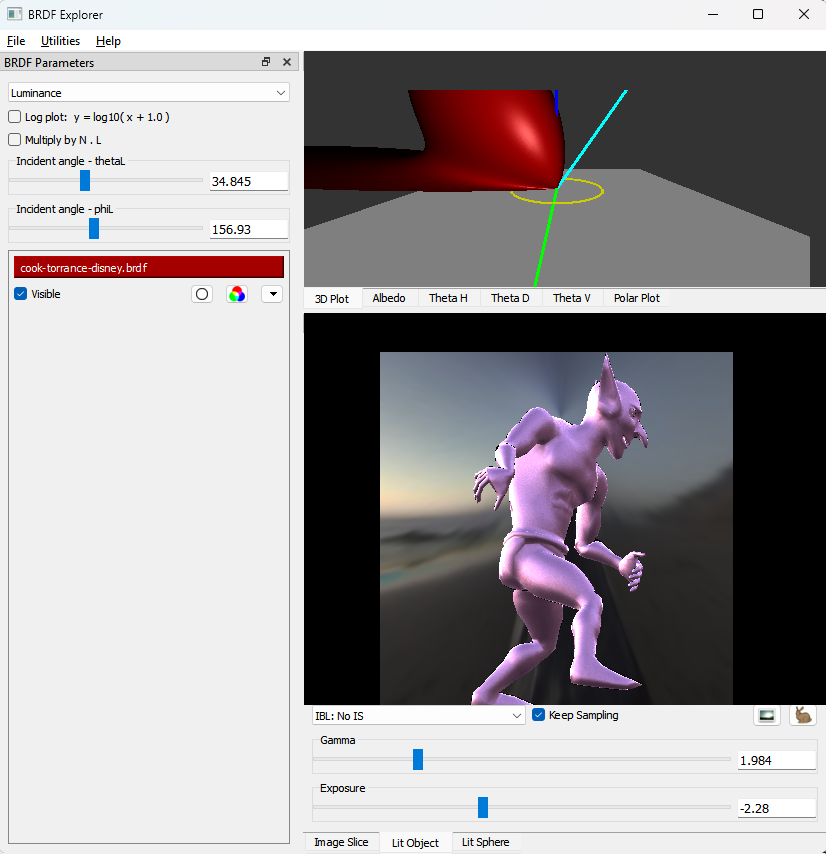
\includegraphics[scale=0.65]{./Imagens/disney-brdf-tool-original.png}
            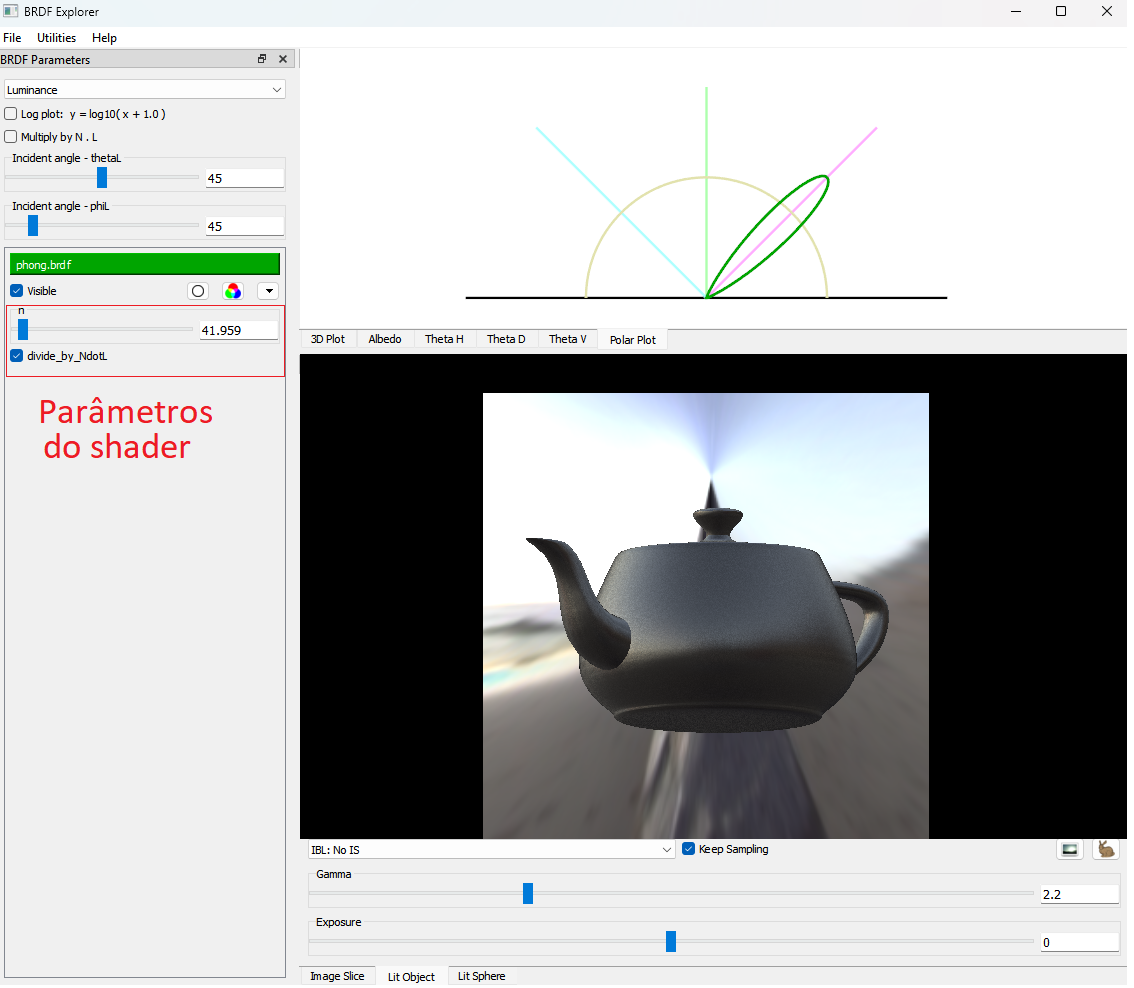
\includegraphics[scale=0.55]{./Imagens/disney-tool-new.png}
        \end{center}
  \legend{ \small Fonte: autor.}
\end{figure}

\begin{codigo}[h]
    \caption{\small \small O código GLSL com sintaxe extra para definir parâmetros. }
    \label{cod-disney-code}
\begin{lstlisting}[language=C, frame=none, inputencoding=utf8]
analytic

# variables go here...
# only floats supported right now.
# [type] [name] [min val] [max val] [default val]

::begin parameters
float n 1 1000 100
bool divide_by_NdotL 1
::end parameters

# Then comes the shader. This should be GLSL code
# that defines a function called BRDF (although you can
# add whatever else you want too, like sqr() below).

::begin shader

vec3 reflect(vec3 I, vec3 N)
{
    return 2*dot(I,N)*N - I;
}

float sqr( float x )
{
    return x*x;
}


// Phong BRDF
vec3 BRDF( vec3 L, vec3 V, vec3 N, vec3 X, vec3 Y )
{
    vec3 R = reflect(L,N);

    // specular
    float val = pow(max(0, dot(R,V)),n);
    if (divide_by_NdotL)
        val = val / dot(N,L);
    return vec3(val);
}
::end shader
\end{lstlisting}
\end{codigo}


